\chapter{Search for H(Inv) decays in the VBF channel with CMS prompt data}
\label{CHAPTER:PromptDataAnalysis}

\glsresetall % Resetting all acronyms

%Status: DONE

In this analysis we focus on Higgs boson decays into invisible particles produced in association with two final state quark jets. These jets will have large rapidity separation and high invariant mass. An event selection criteria has been developed to take advantage of this distinct topology, by selecting two jets with \gls{VBF} characteristics and large \gls{MET} in order to separate signal from other background processes. We have drawn inspiration from the selection criteria proposed in \cite{ARTICLE:Zeppenfeld_ObservingAnInvisibleHiggsboson}.

The main backgrounds for this analysis are from $\Z (\nu \nu)\text{+jets}$ and $\PW (\ell \nu)\text{+jets}$, where the the lepton was not reconstructed or properly identified. These backgrounds are estimated from yields in control regions where we select each boson decay into charged leptons together with a dijet with \gls{VBF} characteristics. These yields are extrapolated to the signal region, using factors determined with the help of \gls{MC} simulation. The background from \gls{QCD} processes is completely estimated from a control regions in data since we cannot rely on \gls{MC} due to insufficient statistics for the extrapolation to the signal region. All other minor backgrounds like from $\ttbar$, single-top, diboson, and Drell--Yan$(\ell\ell)\text{+jets}$ processes are estimated directly from \gls{MC}. 

The observed data yield together with the estimations of the yields for the signal and backgrounds, allow us to perform a single counting experiment and draw limits on the Higgs branching fraction to invisible.

%%%%%%%%%%%%%%%%%%%%%%%%%%%%%%%%%%%%%%%%%%%%%%%%%%%%%%%%%%%%%%%%%%%%%%%%%%%%%%%%%%%%
%%% SECTION
%%%%%%%%%%%%%%%%%%%%%%%%%%%%%%%%%%%%%%%%%%%%%%%%%%%%%%%%%%%%%%%%%%%%%%%%%%%%%%%%%%%%
\section{Event Selection}
\label{SECTION:PromptDataAnalysis_EventSelection}

%Status: DONE

%QUESTION: Was it METnoMu for trigger weights? 
%ANSWER  : yes

%TOPIC: Trigger definition and MC trigger weights
In this analysis we use the recorded data by a purpose designed trigger that selects events with at least one dijet with \gls{VBF} characteristics and \gls{MET}. The dijet is required to have its jets in opposite sides of the detector and pass $\pt^{jet_1},\pt^{jet_2} > 40\,\GeV$, $\Delta\eta > 3.5$ and $M_{jj} > 800\,\GeV$. By requiring any dijet instead of the leading dijet we avoid rejecting events where a \gls{PU} jet is the leading jet or the effects of the lower energy resolution of the trigger versus offline. We also require $MET_{no-\mu} > 65\,\GeV$, the use of \gls{MET} without muons allows us to record with the same trigger, a control sample of processes  $\PW(\mu\nu)\text{+jets}$ and $\Z(\mu\mu)\text{+jets}$. The \gls{MC} simulated events are re-weighted according to the probability of passing the trigger. The trigger weights are determined in a dataset of event recorded with trigger condition requiring a single muon. They are a function of the offline measurements of sub-leading jet \pt, $M_{jj}$ and $MET_{no-\mu}$.

%TOPIC: Signal event selection
The signal region is defined by selecting events with a tighter version of the trigger conditions with additional cuts and vetoes. Building on the trigger requirements we select events where the leading pair of particle flow \cite{ARTICLE:CMSParticleFlowEventRecontruction} anti-$k_T^{\Delta R=0.5}$ jets have $\pt^{jet_1},\pt^{jet_2} > 50\,\GeV$, $|\eta| < 4.7$, $\eta_{jet1} \cdot \eta_{jet2} < 0$, $\Delta\eta_{jj}>4.2$, $M_{jj}>1100\,\GeV$ and large missing energy of at least $130\,\GeV$. We veto events with identified veto electrons or loose muons, as defined in chapter \ref{CHAPTER:EventReconstructionAndSimulation}, to suppress processes with $Z$ or $W$ boson decays. To reduce \gls{QCD} multi-jet backgrounds we additional request the dijet to pass $\Delta\phi < 1.0\,\radian$, since typically \gls{QCD} jets will be back to back and therefore will have high values for this variable. Finally, we require a \acrfull{CJV}, where no additional jet can be present between the two leading jets with $\pt > 30\,\GeV$.

%TOPIC: Selection optimization
The event selection was optimized by setting the lepton vetoes to the recommends values by the relevant \gls{POG} and the \gls{CJV} to a value where its behaviour is well understood. All other thresholds were optimised to obtain the best possible signal significance which was calculated with a profile likelihood method that takes into consideration all relevant systematics. In the calculation the Higgs mass was assumed to be $125\,\GeV$ and a branching ration to invisible of 100\%. The variables involved in the trigger (jet \pt, $M_{jj}$ and \gls{MET}) are constrained to be above the 95\% efficiency working point of the trigger. Distributions of the selected dijet $M_{jj}$, $\Delta\eta$, $\Delta\phi$ and of the \gls{CJV} for \gls{MC} simulation are shown on figure \ref{FIGURE:PromptDataAnalysis_EventSelection_KeyVariables} together with the optimized cut thresholds.

\begin{figure}[!htb]
\centering
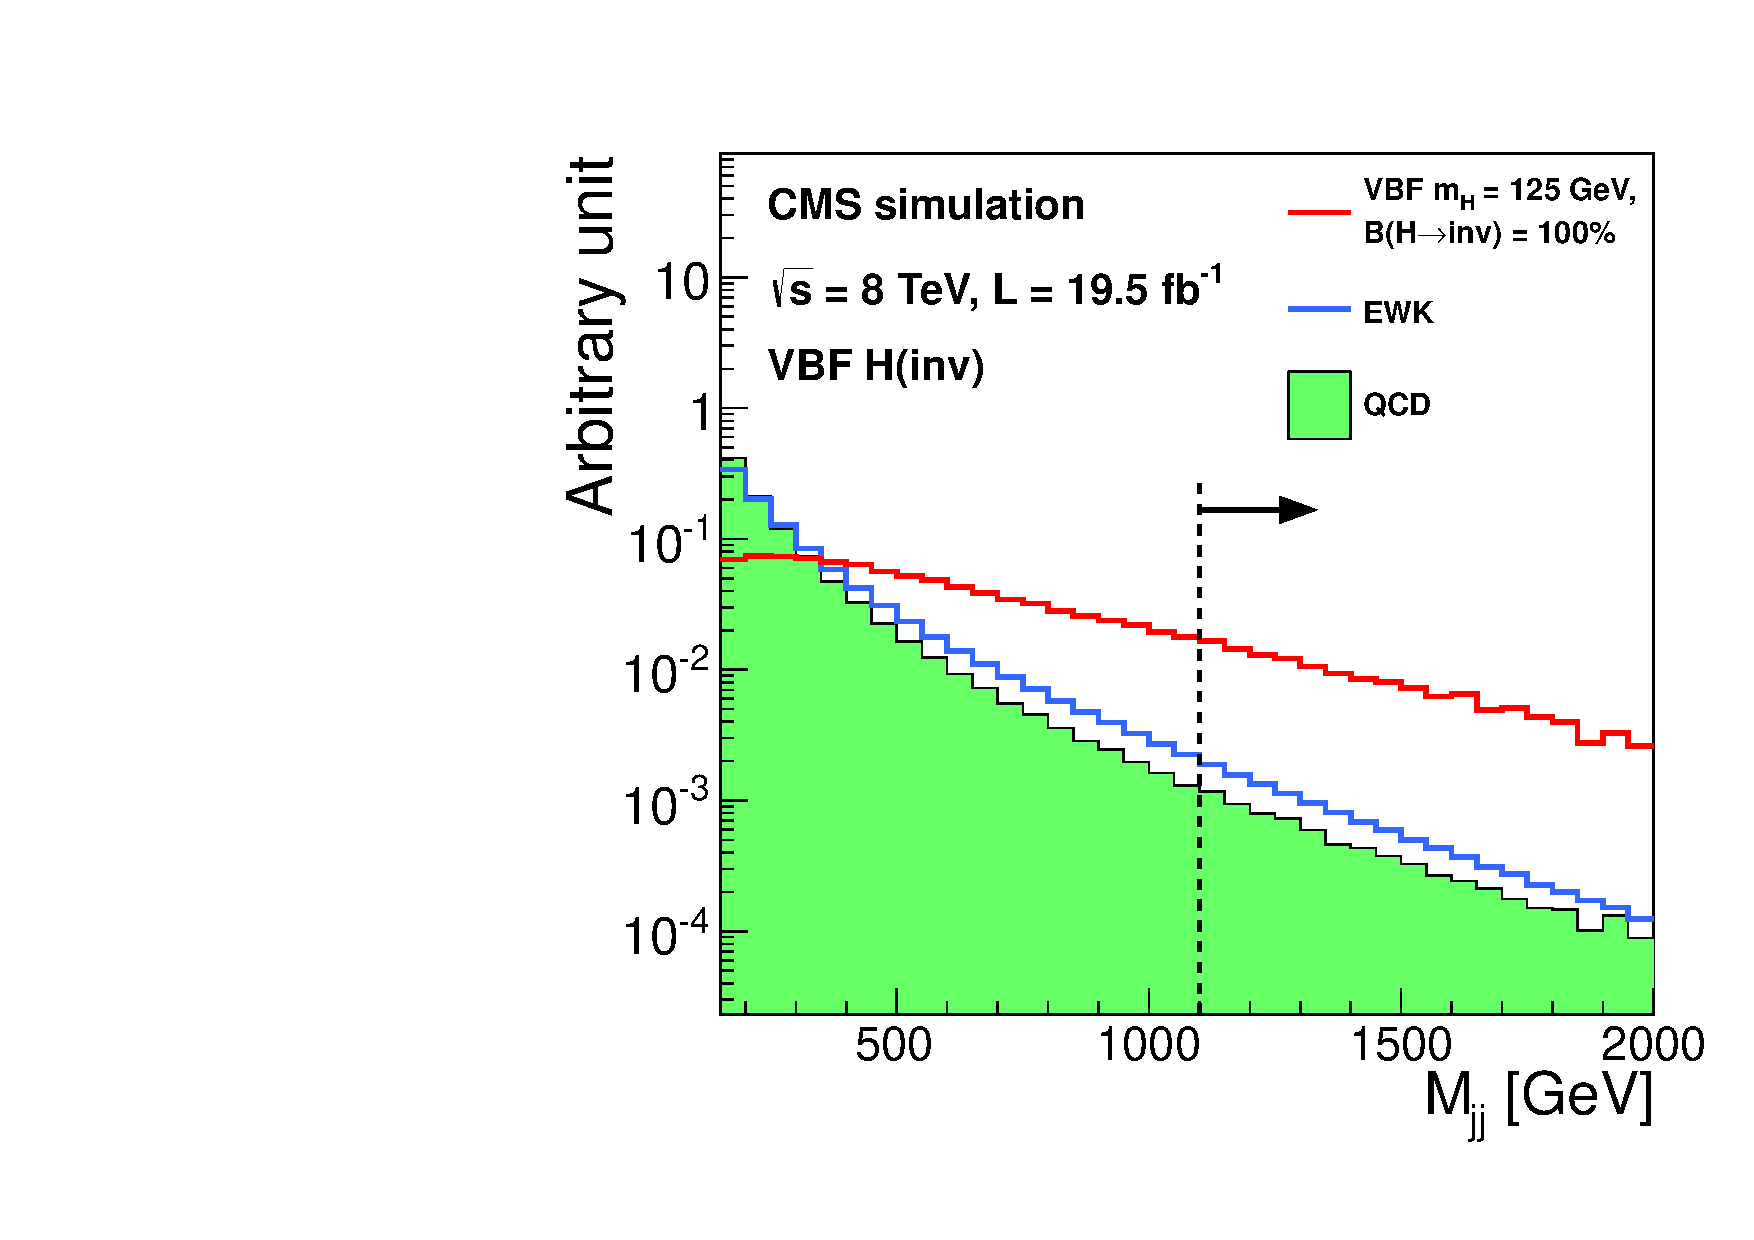
\includegraphics[width=0.49\textwidth]{Chapter05/Images/VBF-Dijet-M.pdf}
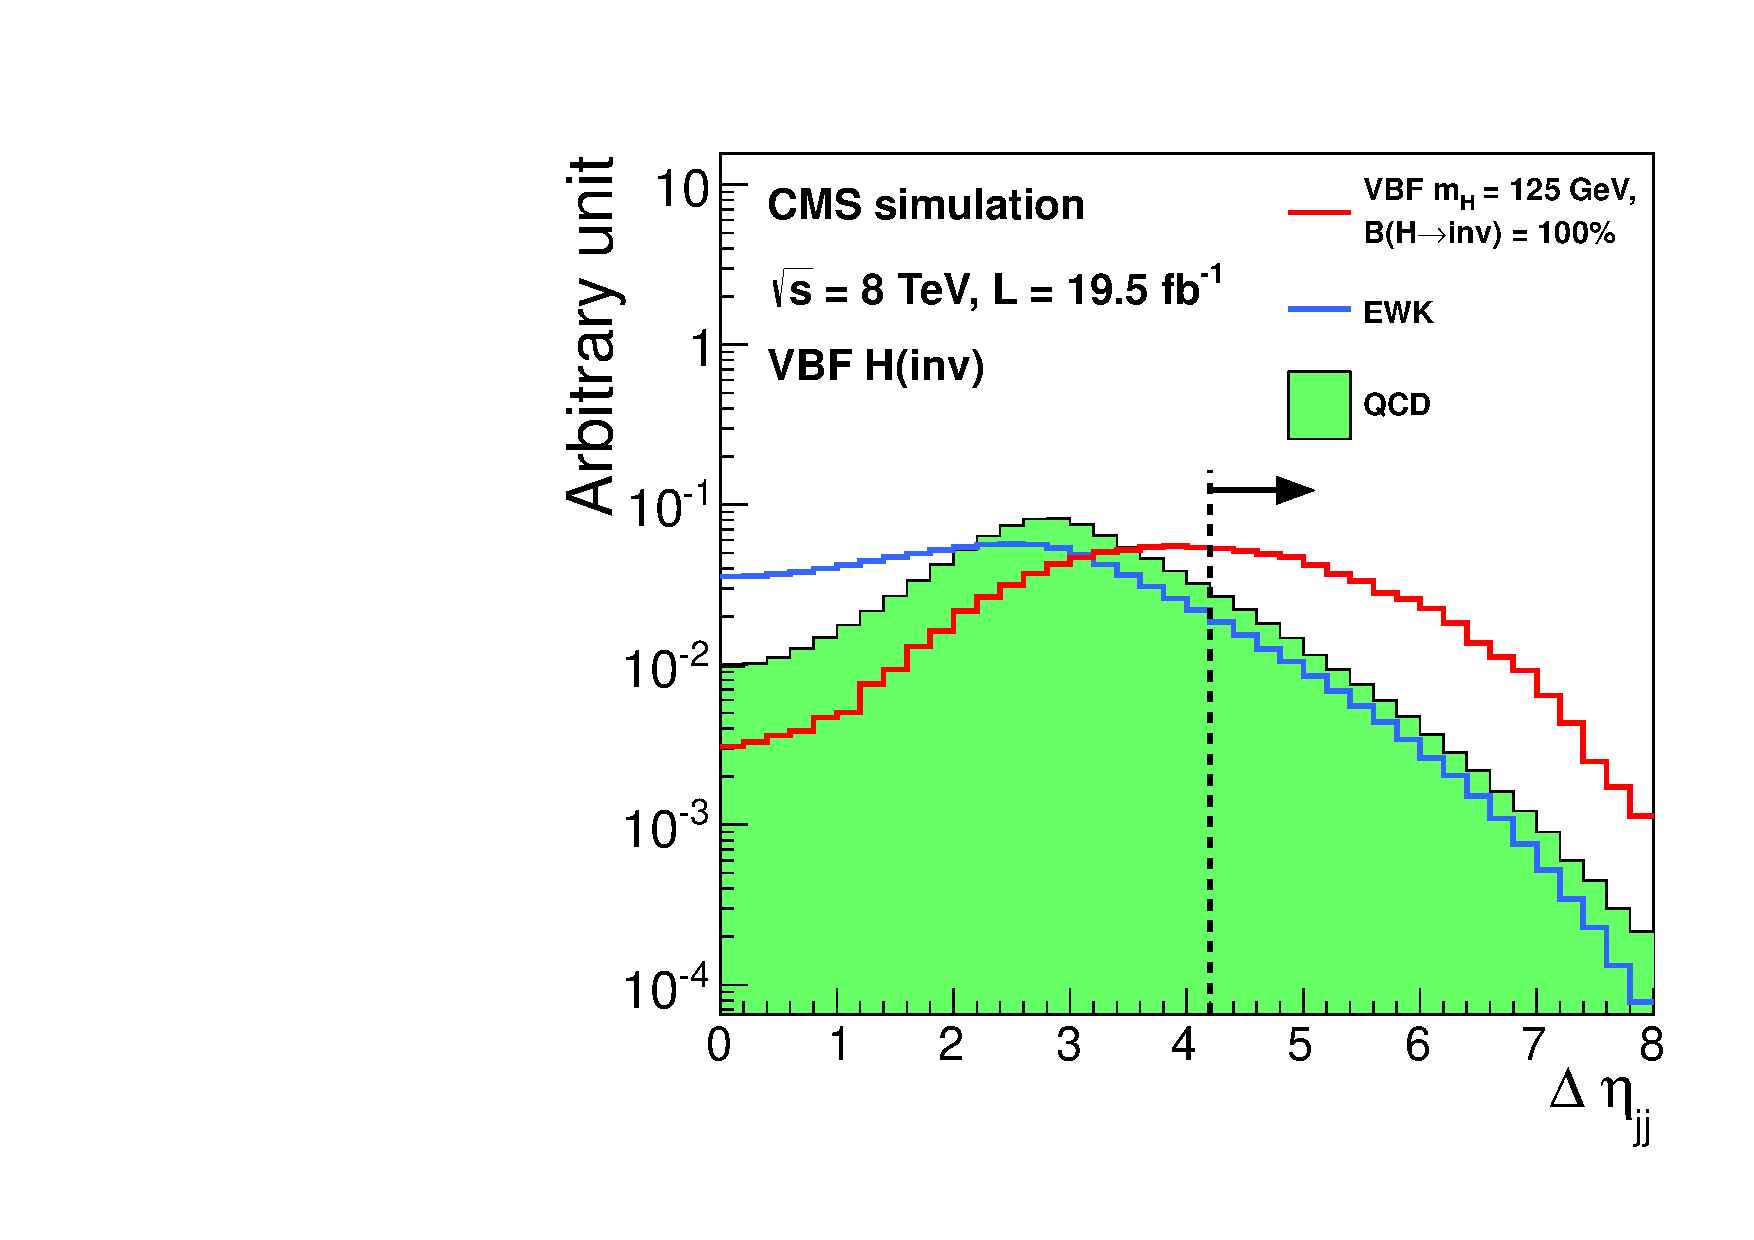
\includegraphics[width=0.49\textwidth]{Chapter05/Images/VBF-Dijet-DEta.pdf}     
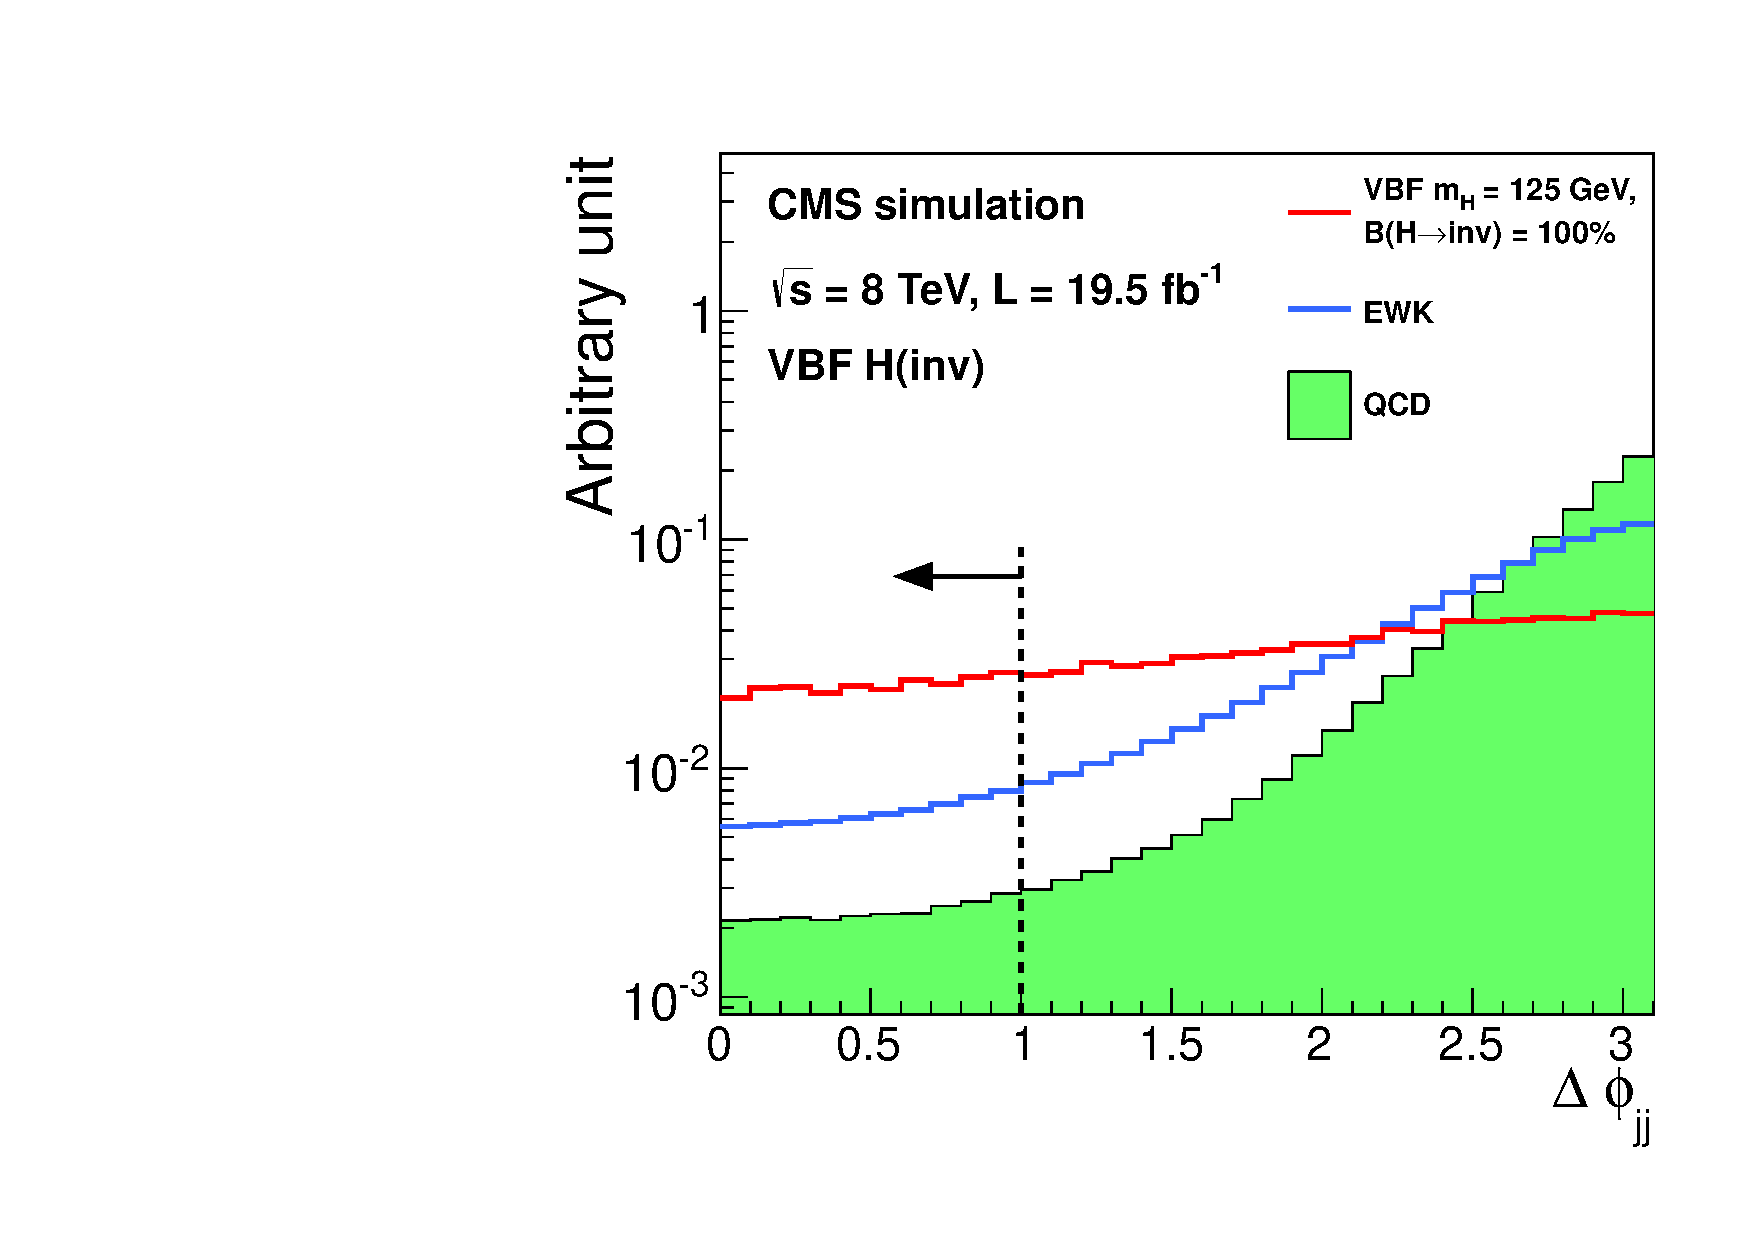
\includegraphics[width=0.49\textwidth]{Chapter05/Images/VBF-Dijet-DPhi.pdf}
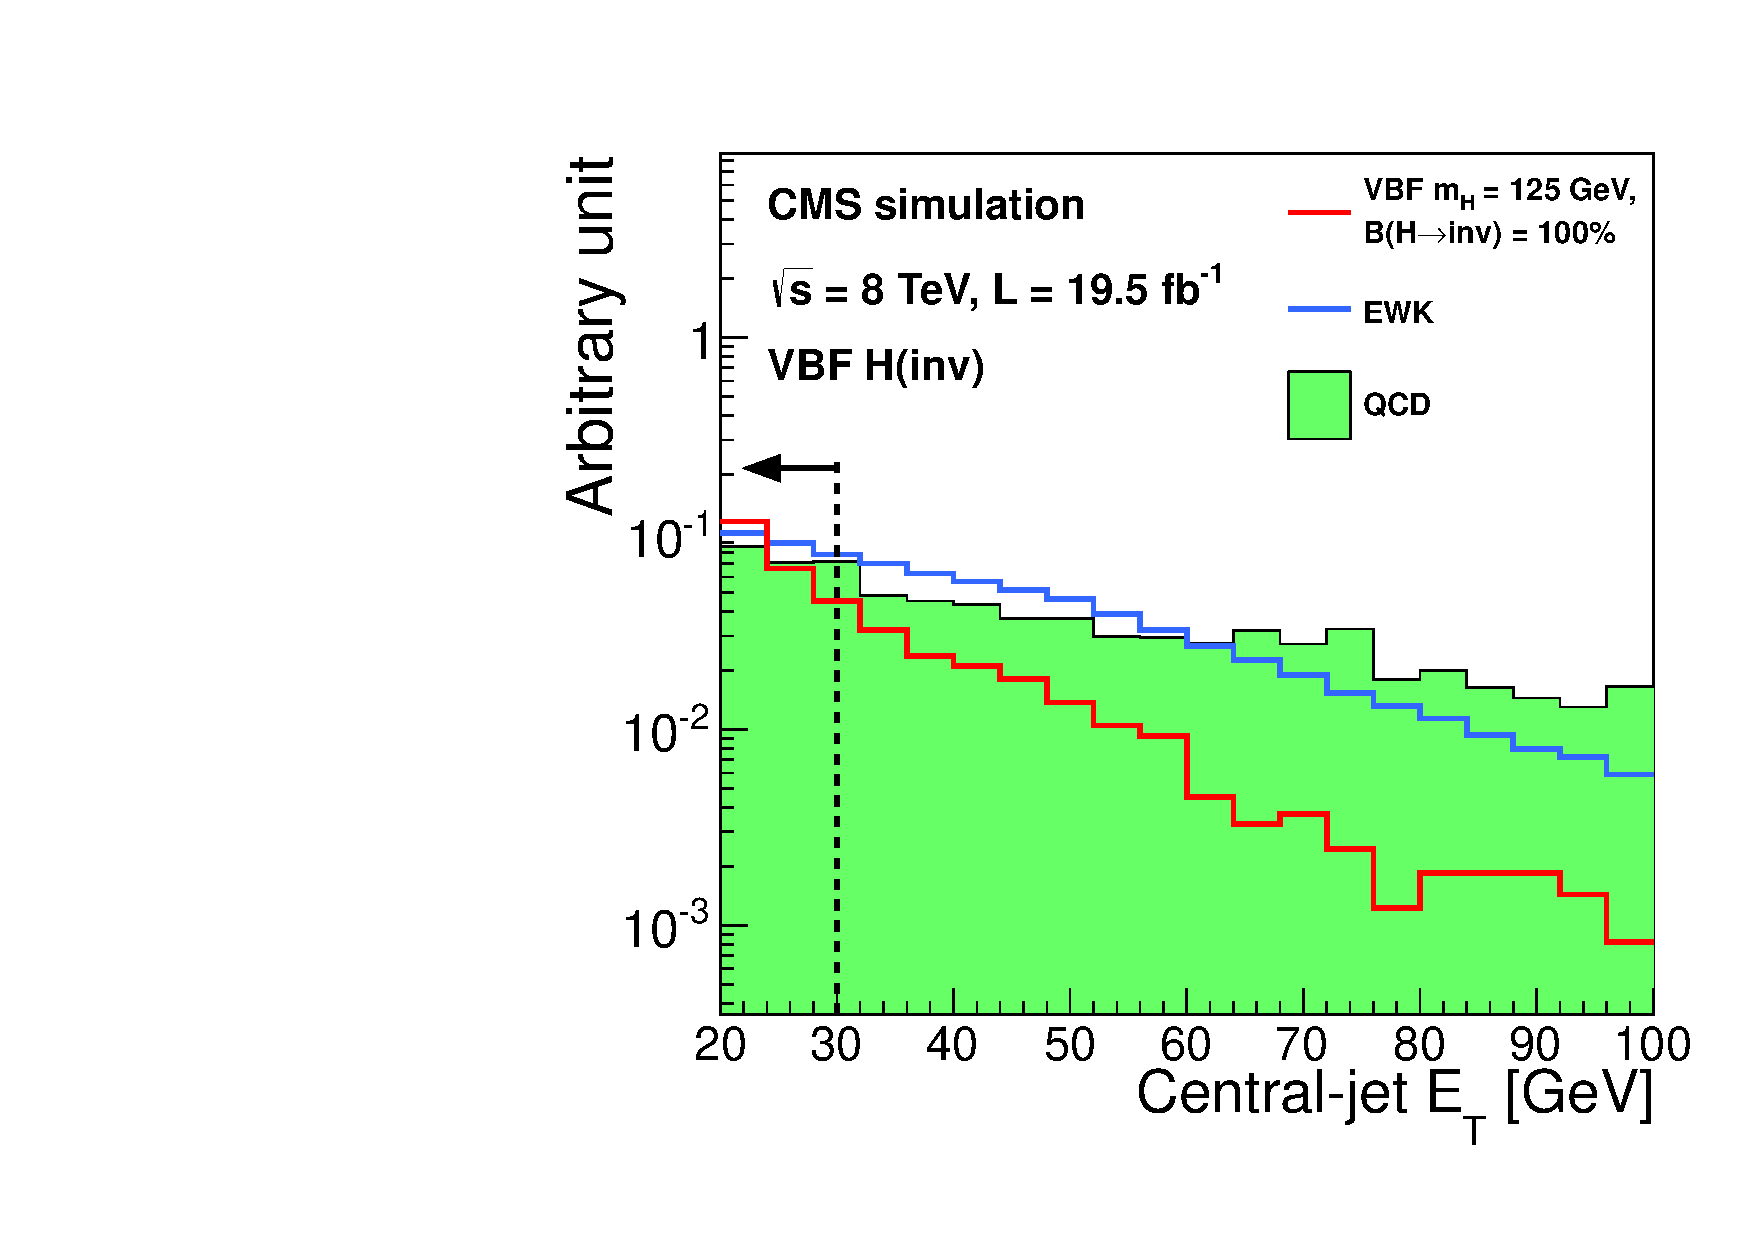
\includegraphics[width=0.49\textwidth]{Chapter05/Images/VBF-CJV-pT.pdf} 
\caption{Distributions of $M_{jj}$ (top left), $\Delta\eta_{jj}$ (top right), $\Delta\phi_{jj}$ (bottom left), and central jet \pt (bottom right) in background and signal MC simulation. The distributions are shown after requiring two jets with $\pt^{jet_1},\pt^{jet_2} > 50\,\GeV$, $|\eta| < 4.7$, $\eta_{jet1} \cdot \eta_{jet2} < 0$, $M_{jj}>150$\GeV, and $MET > 130\,\GeV$. The arrows correspond to the thresholds applied for the final selection, after optimization. \cite{ARTICLE:CMSVBFHiggsToInvAndZHCombination}}
\label{FIGURE:PromptDataAnalysis_EventSelection_KeyVariables}
\end{figure}

To estimate the signal yields the \textsc{POWHEG} \gls{MC} generator was used to create events with a Higgs boson produced via the \gls{VBF} channel with \gls{SM} couplings and with mass of $125\,\GeV$. The obtained signal efficiency was $(6.8 \pm 0.3) \times 10^{-3}$, which corresponds to an event yield of $210 \pm 29\syst$. The signal efficiency dependency on jet $\pt$, dijet $M_jj$, and \gls{MET} is correlated and of comparable amounts. Additionally, a small amount of gluon-fusion signal, where \gls{ISR} take the role of the \gls{VBF} jets, is also expected to pass the signal event selection. Using the same \gls{MC} event generator this contribution has been estimated to be of $14 \pm 10\syst$ events.

%%%%%%%%%%%%%%%%%%%%%%%%%%%%%%%%%%%%%%%%%%%%%%%%%%%%%%%%%%%%%%%%%%%%%%%%%%%%%%%%%%%%
%%% SECTION
%%%%%%%%%%%%%%%%%%%%%%%%%%%%%%%%%%%%%%%%%%%%%%%%%%%%%%%%%%%%%%%%%%%%%%%%%%%%%%%%%%%%
\section{Background Estimation}

%Status: Writing

The irreducible background $\Z(\nu \nu)\text{+jets}$ is estimated from data using as proxy $\Z (\mu \mu)$ decays. 


% The $\Z(\nu \nu)\text{+jets}$ background is estimated from data using observable $\Z (\mu \mu)$ decays. We define a \Z\ control region as for the signal region, with the following changes to the event selection: the lepton veto is replaced with a requirement of an oppositely charged pair of well reconstructed and isolated muons each with $\pt > 20 $\GeV, and invariant mass $60 < M_{\mu\mu}<120$\GeV, a veto is applied on any additional leptons with $\pt>10$\GeV, and the $\ETm$ is recomputed after removing the muons from the \Z\ boson decay. The number of $\Z (\nu \nu)$ events in the signal region is then predicted using:

% \begin{equation}
% N^\mathrm{s}_{\nu\nu} = (N^\mathrm{c}_{\mu\mu\text{obs}} - N^\mathrm{c}_\text{bkg}) \cdot \frac{\sigma(\Z \to \nu\nu)}{\sigma(\Z/\gamma^{*} \to \mu\mu)} \cdot \frac{\varepsilon^\mathrm{s}_{\Z \mathrm{MC}}}{\varepsilon^\mathrm{c}_{\Z \mathrm{MC}}}.
% \end{equation}
% 

\begin{figure}[!htb]
\centering
\includegraphics[width=0.45\textwidth]{Chapter05/Images/ZCtrlMET.pdf}
\includegraphics[width=0.45\textwidth]{Chapter05/Images/ZCtrlMjj.pdf}   
\caption{The $MET$ (left plot) and $M_{jj}$ (right plot) distributions in the relaxed $Z$ control region of the \gls{VBF} search, with no requirements on $\Delta\eta_{jj}$, $\Delta\phi_{jj}$, or \gls{CJV}, and with the $M_{jj}$ requirement relaxed to $1000\,\GeV$.  The simulated background from different processes is shown cumulatively, and normalized to the data, with its systematic uncertainty shown as a hatched region.  The lower panels show the ratio of data to the simulated background, again with the systematic uncertainty shown as a hatched region. \cite{ARTICLE:CMSVBFHiggsToInvAndZHCombination}}
\label{fig:zCtrl}
\end{figure}

\begin{table}[!htb]
\centering
\begin{tabular}{|l|c|}
\hline
Process                                  & Event yields                  \\
\hline
$\Z (\nu\nu)\text{+jets}$                & $  99 \pm  29 \stat \pm 25 \syst$  \\
$\PW (\mu\nu)\text{+jets}$               & $  67 \pm   5 \stat \pm 16 \syst$   \\
$\PW (\Pe \nu)\text{+jets}$              & $  63 \pm   9 \stat \pm 18 \syst$   \\
$\PW (\tauh \nu)\text{+jets}$            & $  53 \pm  18 \stat \pm 18 \syst$  \\
QCD multijet                             & $  31 \pm   5 \stat \pm 23 \syst$   \\
Sum (\ttbar, single top quark, $VV$, DY) & $20.0 \pm 8.2 \syst$ \\
\hline\hline
Total background                         & $332 \pm 36 \stat \pm 45 \syst$ \\
VBF H(inv.)                              & $210 \pm 29 \syst$ \\
ggF H(inv.)                              & $ 14 \pm 10 \syst$ \\
Observed data                            & 390  \\
\hline\hline
S/B                                      & 70\% \\
\hline
\end{tabular}
\label{tab:bgSummary}
\caption{Summary of the estimated number of background and signal events, together with the observed yield, in the VBF search signal region.  The signal yield is given for $m_H=125$\GeV and $\BRinv=100$\%. \cite{ARTICLE:CMSVBFHiggsToInvAndZHCombination}}
\end{table}

% \subsection{Background estimation}
% \label{sec:vbf-backgrounds}
% 

% The ratio of cross sections, $\sigma(\Z \to \nu \nu) / \sigma(\Z/\gamma^{*} \to \mu \mu) = 5.651 \pm 0.023\syst$ is calculated with \MCFM~\cite{MCFM} for $m_{\Z/\gamma^{*}} > 50$\GeV, the mass range of the MC sample.  The selection efficiencies in the signal region, $\varepsilon^\mathrm{s}_{\Z \mathrm{MC}} = (1.65 \pm 0.27\syst) \times 10^{-6}$, and the control region, $\varepsilon^\mathrm{c}_{\Z \mathrm{MC}}=(1.11 \pm 0.17\syst) \times 10^{-6}$, are estimated from DY($\ell\ell$)+jets simulation, ignoring the muons when computing the efficiency in the signal region.
% The observed yield in the control region is $N^\mathrm{c}_{\mu\mu\text{obs}} = 12$~events.  The background in the control region---estimated from $\ttbar$, diboson and single-top MC samples---is $N^\mathrm{c}_\text{bkg}=0.23 \pm 0.15\syst$~events.  The resulting estimate of the $\Z (\nu \nu)$ background in the signal region is $99 \pm 29\stat \pm 25\syst$ events.  The source of systematic uncertainty in the background estimates will be described in Section~\ref{sec:vbf-syst}.
% Figure~\ref{fig:zCtrl} shows the $\ETm$ and dijet invariant mass, $\mjj$, distributions with a relaxed set of criteria for the \Z control region, with $\mjj>1000$\GeV and no requirements on $\etajj$, $\phijj$, or CJV.  In this figure, the simulated background is normalized to the data.  It should be noted that our estimates of the dominant V+jets background are insensitive to the overall normalization of the simulation, which cancels in the ratio.
% 
% \begin{figure}[hbtp]
%         \begin{center}
%                  \includegraphics[width=0.45\textwidth]{ZCtrlMET.pdf}
%                  \includegraphics[width=0.45\textwidth]{ZCtrlMjj.pdf}   
%                 \caption{The $\ETm$ (\cmsLeft) and $\mjj$ (\cmsRight) distributions in the relaxed \Z control region of the VBF search, with no requirements on $\etajj$, $\phijj$, or CJV, and with the $\mjj$ requirement relaxed to 1000\GeV.  The simulated background from different processes is shown cumulatively, and normalized to the data, with its systematic uncertainty shown as a hatched region.  The lower panels show the ratio of data to the simulated background, again with the systematic uncertainty shown as a hatched region.}
%                 \label{fig:zCtrl}
%         \end{center}
% \end{figure}
% 
% 
% The $\PW (\Pe \nu)\text{+jets}$ and $\PW (\mu \nu)\text{+jets}$ backgrounds are estimated from single-lepton control samples.
% We define $\PW (\mu \nu)$ and $\PW (\Pe \nu)$ control regions in a similar way to the \Z\ boson background.  In the $\PW (\mu \nu)$ region, the lepton veto is replaced with a single $\mu$ requirement and a veto on any additional leptons, and the $\ETm$ is recomputed after removing the muon from the \PW\ boson decay.  The $\PW (\Pe \nu)$ region is defined similarly, with a single electron requirement and additional lepton veto, but here the $\ETm$ is not recomputed, since the electron energy is already included in the $\ETm$ at trigger level.  The number of $\PW (\ell \nu)$ (where ${\ell=\Pe,\mu}$) events in the signal region, $N^\mathrm{s}_{\ell}$ is then estimated using:
% \begin{equation}
%         \label{eq:w}
% N^\mathrm{s}_\ell = (N^\mathrm{c}_{\ell\text{obs}} - N^\mathrm{c}_\text{bkg}) \cdot \frac{N^\mathrm{s}_{\PW \mathrm{MC}}}{N^\mathrm{c}_{\PW \mathrm{MC}}},
% \end{equation}
% where $N^\mathrm{s}_{\PW \mathrm{MC}}$ and $N^\mathrm{c}_{\PW \mathrm{MC}}$ are the number of events in the signal and control regions in the $\PW (\ell \nu)\text{+jets}$ MC simulation.  The ratio $N^\mathrm{s}_{\PW \mathrm{MC}}/N^\mathrm{c}_{\PW \mathrm{MC}}$ is equal to $0.347 \pm 0.045\syst$ for $\PW (\mu \nu)$ and $1.08 \pm 0.21\syst$ for $\PW (\Pe \nu)$. In the $\PW (\mu \nu)$ control region the observed yield is 223 events, with a background of $30.4 \pm 7.0\syst$ events.  The observed yield in the $\PW (\Pe \nu)$ control region is 65 events, with a background of $7.1 \pm 4.7\syst$ events.  The $\PW (\mu \nu)$ background in the signal region is then estimated to be $66.8 \pm 5.2\stat \pm 15.7\syst$ events, and the $\PW (\Pe \nu)$ background to be $62.7 \pm 8.7\stat \pm 18.1\syst$ events.
% 
% The background arising from $\PW (\tau \nu)\text{+jets}$, where the tau lepton decays hadronically ($\tauh$) is estimated using a slightly different method, since a tau lepton veto is not applied in the invisible Higgs boson signal selection.  Hadronically decaying taus are reconstructed using the ``hadron plus strips'' algorithm~\cite{Chatrchyan:2012zz}. This uses charged hadrons and neutral electromagnetic objects (photons) to reconstruct hadronic tau decay modes with one or three charged particles, in the range $\abs{\eta} < 2.3$. A control region is defined, requiring one hadronic tau with $\pt>20$\GeV and $\abs{\eta}<2.3$, no additional leptons, and the remaining signal region selection. However, in the $\PW (\tauh \nu)$ control region, the CJV is not applied in order to increase the yield.  The number of $\PW (\tauh \nu)$ events in the signal region, $N^\mathrm{s}_{\tauh}$, is then estimated from the control region in the same way as the $\PW (\mu \nu)$ and $\PW (\Pe \nu)$ backgrounds. A yield of 32 events is observed in the control region, with the background estimated from the MC simulation to be $15.2 \pm 3.6\syst$ events, giving an estimate of the $\PW (\tauh \nu)$ background in the signal region of $53 \pm 18\stat \pm 18\syst$ events.
% 
% % \begin{equation}
% %       \label{eq:wtau}
% % N^\mathrm{s}_{\tauh} = (N^\mathrm{c}_{\tau\text{obs}} - N^\mathrm{c}_\text{bkg}) \cdot \frac{\varepsilon_\mathrm{CJV}}{\varepsilon_{\tau}},
% % \end{equation}
% 
% %and the efficiency of the tau control region selection, $\varepsilon_{\tau}$ is $0.134 \pm 0.023\syst$.
% 
% In order to cross check the backgrounds from V+jets processes (where V represents either a \PW\ or a \Z boson), which dominate in the signal region, the $\PW (\mu \nu)$ control region and MC simulation is used to compute yields in other control regions. For example, the yield in the $\Z (\mu \mu)$ region is given by:
% \begin{equation}
%         \label{eq:zfromw}
% N^\mathrm{c}_{\mu \mu} = (N^\mathrm{c}_{\mu \text{obs}} - N^\mathrm{c}_\text{bkg}) \cdot \frac{N^\mathrm{c}_{\Z \mathrm{MC}}}{N^\mathrm{c}_{\PW \mathrm{MC}}},
% \end{equation}
% 
% Similar expressions are used to estimate yields in the $\PW (\Pe \nu)$ and $\PW (\tauh \nu)$ control regions. In all cases, the predictions from data agree with the observed yield within the uncertainty.
% 
% The QCD multijet background in the signal region is estimated using the fractions of events passing the $\ETm$ and CJV requirements.  We define regions A, B, C, and D as follows, after the full remaining selection :
% 
% \begin{itemize}
%         \item{A: fail $\ETm$ selection, fail CJV selection;}
%         \item{B: pass $\ETm$ selection, fail CJV selection;}
%         \item{C: fail $\ETm$ selection, pass CJV selection;}
%         \item{D: pass $\ETm$ selection, pass CJV selection.}
% \end{itemize}
% 
% We estimate the QCD multijet component in regions A, B, and C from data, after subtracting the electroweak backgrounds using estimations from simulation.  The QCD multijet component in the signal region D can then be estimated using $N_\mathrm{D} = N_\mathrm{ B}N_\mathrm{C} / N_\mathrm{A}$, where $N_{i}$ is the number of events in region $i$.  This method is based on the assumption that the $\ETm$ and the CJV are uncorrelated, which has been checked by comparing the $\ETm$ distribution, below the 130\GeV threshold, in events passing and failing the CJV.  The maximum difference in the $\ETm$ distribution between these two samples is 40\%, which is assigned as a systematic uncertainty of the method.  We predict the QCD background in the signal region to be $30.9 \pm 4.8\stat \pm 23.0\syst$ events.  Furthermore, the method is tested on a high statistics sample with selections equivalent to those in the signal region, but dominated by QCD multijet events by changing the $\phijj$ requirement to $\phijj>2.6$~radians.  In this sample, we observe $2551 \pm 57\stat$ events in the pseudo-signal region after subtraction of backgrounds, which are estimated from MC simulation.  The QCD multijet component is predicted to be $2959 \pm 58\stat$, which is compatible with the observation within the systematic uncertainty.  To give further confidence in this estimate, we perform a cross-check using an ABCD method based on the $\ETm$ and $\phijj$ variables, which gives a prediction consistent with the main method.
% 
% The remaining SM backgrounds in the signal region---due to $\ttbar$, single-top, VV and DY($\ell\ell$)+jets---are estimated from MC simulation to be $20.0 ^{+6.0}_{-8.2}\syst$ events.  The total expected background is $332 \pm 36\stat \pm 45\syst$.  The background estimates are summarised in Table~\ref{tab:bgSummary} along with the expected yield for a signal with $\mH=125$\GeV and $\BRinv=100$\%.
% 
% \begin{table}[!htb]
% \centering
% \begin{tabular}{lc}
% \hline \hline
% Process                                                 & Event yields \\
% \hline$\Z (\nu\nu)\text{+jets}$          & $99 \pm 29\stat \pm 25\syst$ \\
% $\PW (\mu\nu)\text{+jets}$               & $67 \pm 5\stat \pm 16\syst$   \\
% $\PW (\Pe \nu)\text{+jets}$              & $63 \pm 9\stat \pm 18\syst$   \\
% $\PW (\tauh \nu)\text{+jets}$            & $53 \pm 18\stat \pm 18\syst$  \\
% QCD multijet                             & $31 \pm 5\stat \pm 23\syst$   \\
% Sum (\ttbar, single top quark, $VV$, DY) & $20.0 \pm 8.2\syst$ \\
% \hline
% Total background                         & $332 \pm 36\stat \pm 45\syst$  \\
% VBF H(inv.)                              & $210 \pm 29\syst$ \\
% ggF H(inv.)                              & $14 \pm 10\syst$ \\
% Observed data                            & 390  \\
% \hline
% S/B                                      & 70\% \\
% \hline \hline
% \end{tabular}
% \label{tab:bgSummary}
% \caption{Summary of the estimated number of background and signal events, together with the observed yield, in the VBF search signal region.  The signal yield is given for $\mH=125$\GeV and $\BRinv=100$\%.}
% \end{table}

%%%%%%%%%%%%%%%%%%%%%%%%%%%%%%%%%%%%%%%%%%%%%%%%%%%%%%%%%%%%%%%%%%%%%%%%%%%%%%%%%%%%
%%% SECTION
%%%%%%%%%%%%%%%%%%%%%%%%%%%%%%%%%%%%%%%%%%%%%%%%%%%%%%%%%%%%%%%%%%%%%%%%%%%%%%%%%%%%
\section{Sources of uncertainty}

%Status: Writing

\begin{table}[!htb]
\centering
\begin{tabular}{|l|c|c|}
\hline
Source                                           & Total background & Signal \\
\hline\hline
Control region statistics                        & 11\%             & -      \\
MC statistics                                    & 11\%             & 4\%    \\
Jet/$E_T^{\text{miss}}$ energy scale/resolution  & 7\%              & 13\%   \\
QCD background estimation                        & 4\%              & -      \\
Lepton efficiency                                & 2\%              & -      \\
Tau ID efficiency                                & 1\%              & -      \\
Luminosity                                       & 0.2\%            & 2.6\%  \\
Cross sections                                   & 0.5--1\%         & -      \\
PDFs                                             & -                & 5\%    \\
Factorization/renormalization scale              & -                & 4\%    \\
Gluon fusion signal modelling                    & -                & 4\%    \\
\hline\hline
Total                                            & 18\%             & 14\%   \\
\hline 
\end{tabular}
\caption{Summary of the uncertainties in the total background and signal yields in the VBF channel. All uncertainties affect the normalization of the yield, and are quoted as the change in the total background or signal estimate, when each systematic effect is varied according to its uncertainties. The signal uncertainties are given for $m_H=125$\GeV and $\BRinv=100$\%. \cite{ARTICLE:CMSVBFHiggsToInvAndZHCombination}}
\label{TABLE:PromptDataAnalysis_SourcesUncertaintySummary}
\end{table}


%%%%%%%%%%%%%%%%%%%%%%%%%%%%%%%%%%%%%%%%%%%%%%%%%%%%%%%%%%%%%%%%%%%%%%%%%%%%%%%%%%%%
%%% SECTION
%%%%%%%%%%%%%%%%%%%%%%%%%%%%%%%%%%%%%%%%%%%%%%%%%%%%%%%%%%%%%%%%%%%%%%%%%%%%%%%%%%%%
\section{Results}

%Status: Writing

\begin{figure}[htp]
\centering
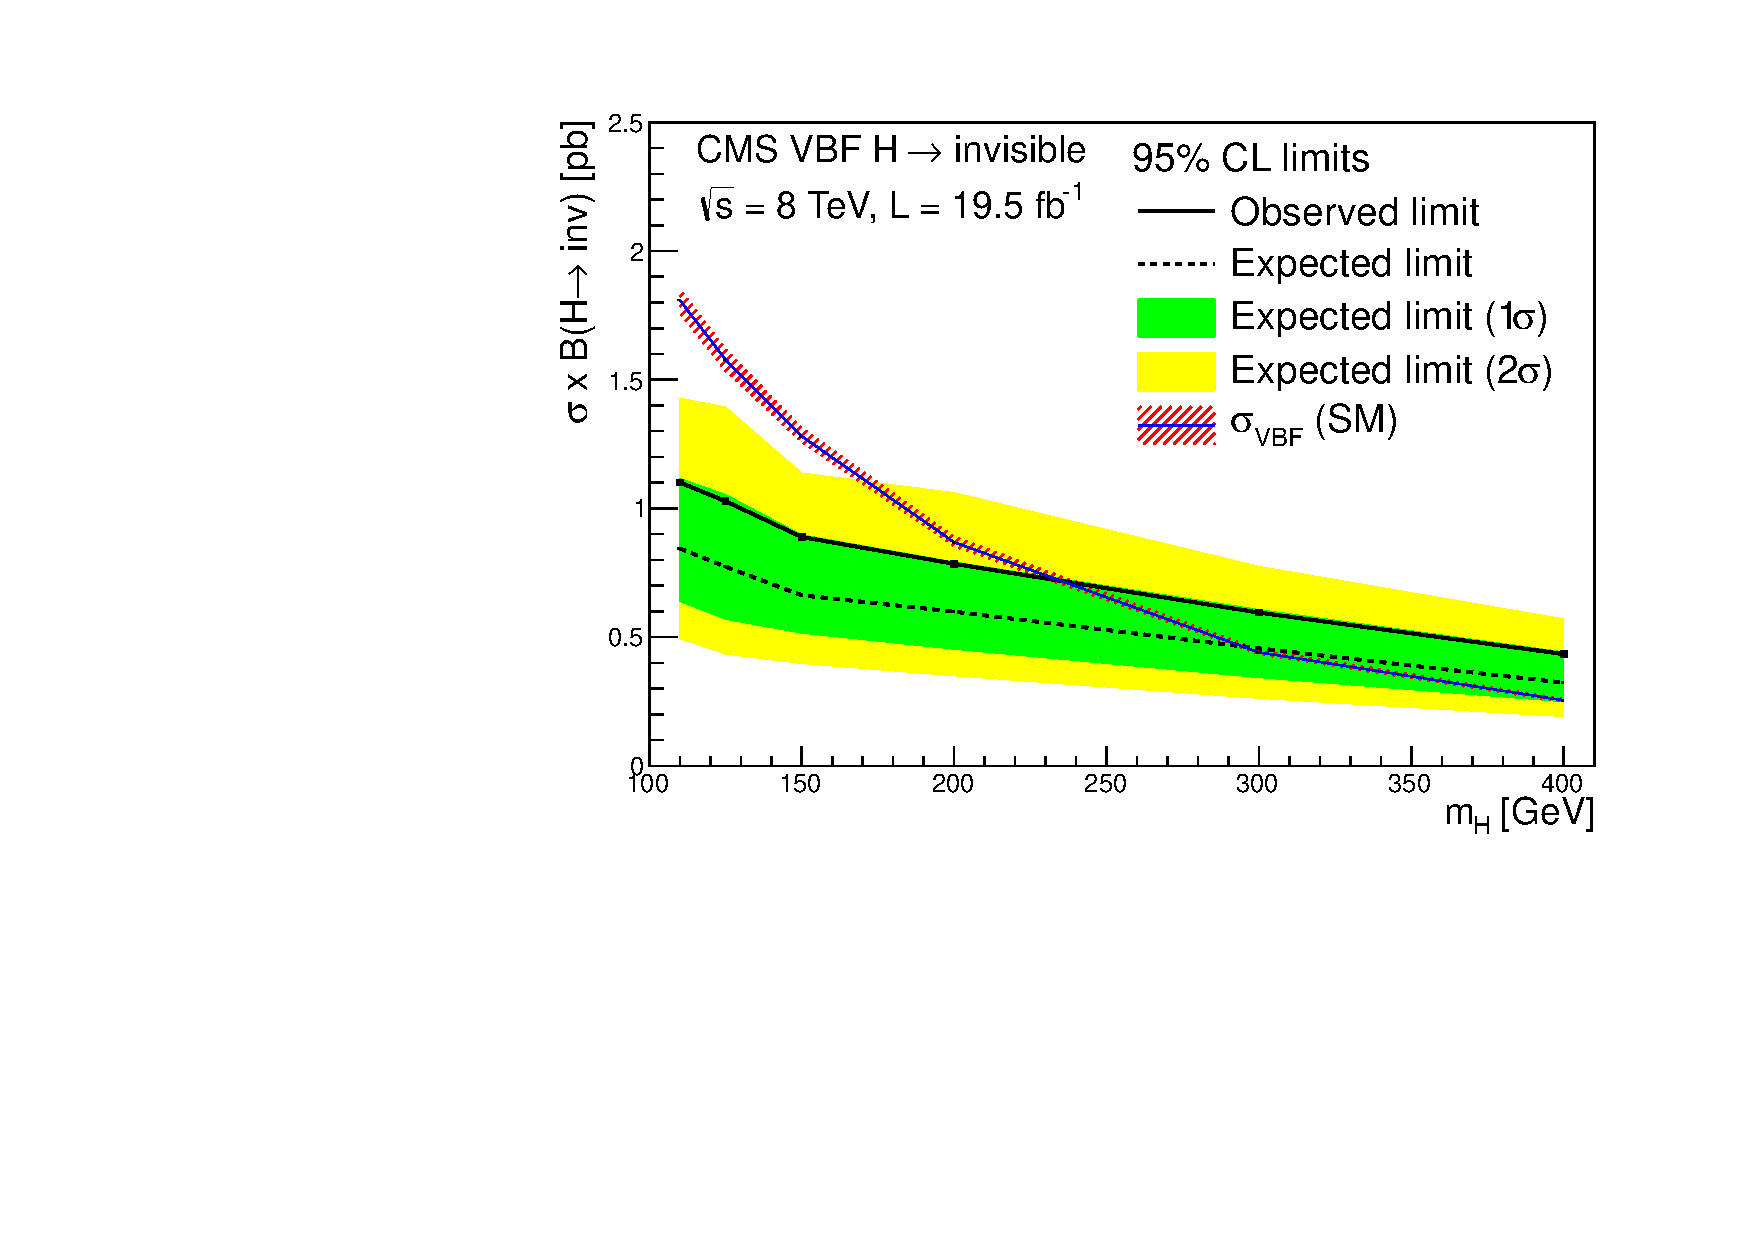
\includegraphics[width=0.49\textwidth]{Chapter05/Images/vbfxslimit.pdf}
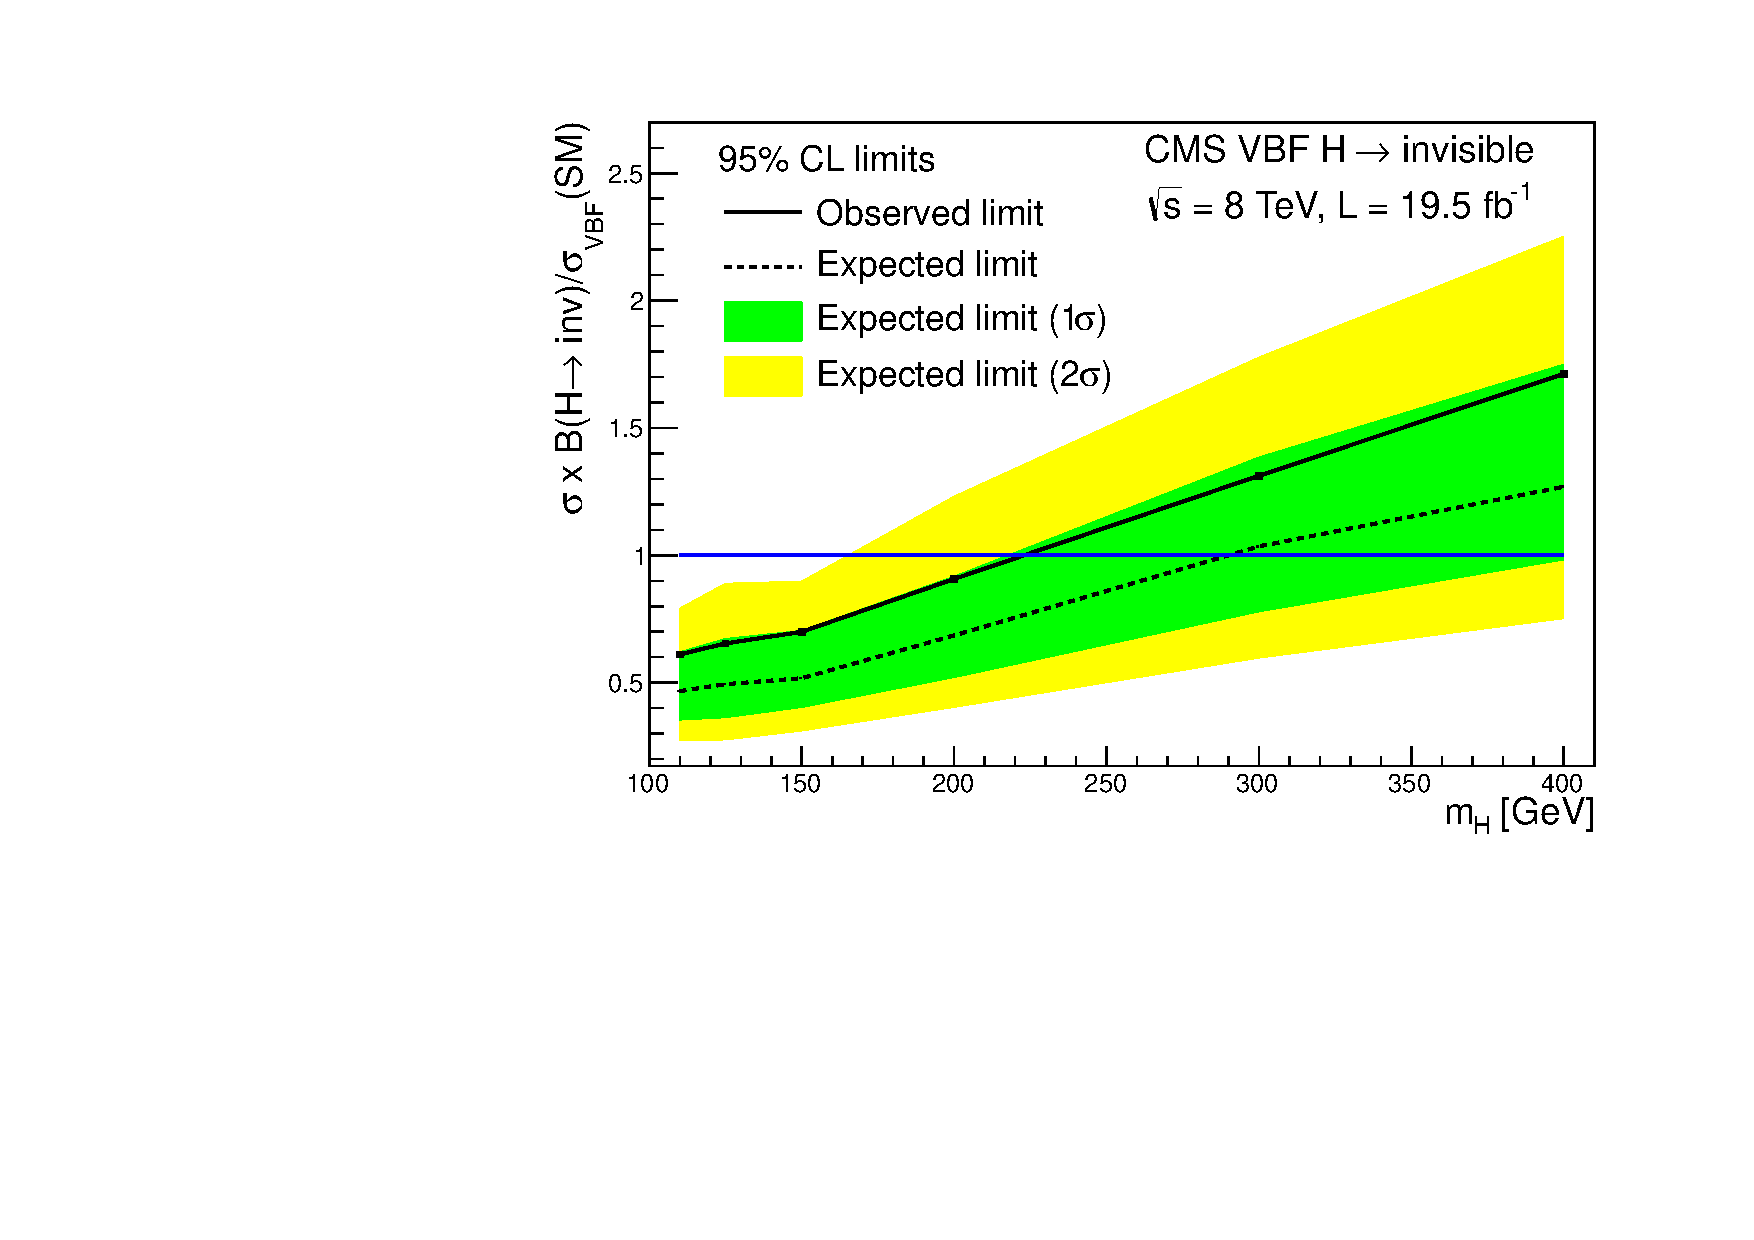
\includegraphics[width=0.49\textwidth]{Chapter05/Images/vbflimit.pdf}
\caption{Expected and observed 95\% CL upper limits on the VBF production cross section times invisible branching fraction (left figure), and normalized to the \gls{SM} Higgs boson \gls{VBF} production cross section (right figure). \cite{ARTICLE:CMSVBFHiggsToInvAndZHCombination}}
\label{FIGURE:vbfLimit}
\end{figure}


%%%%%%%%%%%%%%%%%%%%%%%%%%%%%%%%%%%%%%%%%%%%%%%%%%%%%%%%%%%%%%%%%%%%%%%%%%%%%%%%%%%%
%%% SECTION
%%%%%%%%%%%%%%%%%%%%%%%%%%%%%%%%%%%%%%%%%%%%%%%%%%%%%%%%%%%%%%%%%%%%%%%%%%%%%%%%%%%%
\section{Conclusion}

%Status: Writing


%%%%%%%%%%%%%%%%%%%%%%%%%%%%%%%%%%%%%%%%%%%%%%%%%%%%%%%%%%%%%%%%%%%%%%%%%%%%%%%%%%%%
%%% SECTION
%%%%%%%%%%%%%%%%%%%%%%%%%%%%%%%%%%%%%%%%%%%%%%%%%%%%%%%%%%%%%%%%%%%%%%%%%%%%%%%%%%%%
\section{Preparing parked analysis}


%%%%%%%%%%%%%%%%%%%%%%%%%%%%%%%%%%%%%%%%%%%%%%%%%%%%%%%%%%%
% Jet topology variables
%%%%%%%%%%%%%%%%%%%%%%%%%%%%%%%%%%%%%%%%%%%%%%%%%%%%%%%%%%%
% 18 Months report was on the Sep 9 2013

%/home/hep/jca10/work/vbfinv/ws04/CMSSW_5_3_11/src/UserCode/ICHiggsTauTau/Analysis/HiggsNuNu/PLOTS_mjj1200_dijetFrac/nunu/MET130/n_vtx_2012_DijetFraction_log.pdf
% Looks like plots are from Jun 25 2013

% FOUND FILE: This is the file used in the plots for the 18 months report
%/home/hep/jca10/work/vbfinv/ws04/CMSSW_5_3_11/src/UserCode/ICHiggsTauTau/Analysis/HiggsNuNu/output_mjj1100_dijetFrac/nunu/MET130/MC_VBF_HToZZTo4Nu_M-120.root

%/vols/cms02/jca10/work/ws01/CMSSW_5_3_11/src/UserCode/ICHiggsTauTau/Analysis/HiggsNuNu/plots/DPhiSIGNAL_CJVpass/dijetMet/dijetFrac_htMET.png
% Looks like plots are from Feb 20 2014

%%%%%%%%%%%%%%%%%%%%%%%%%%%%%%%%%%%%%%%%%%%%%%%%%%%%%%%%%%%
% Track variables
%%%%%%%%%%%%%%%%%%%%%%%%%%%%%%%%%%%%%%%%%%%%%%%%%%%%%%%%%%%
% 20140603_ICVBFHiggs_JPela.pdf

%%%%%%%%%%%%%%%%%%%%%%%%%%%%%%%%%%%%%%%%%%%%%%%%%%%%%%%%%%%
% QCD VFB + MET samples
%%%%%%%%%%%%%%%%%%%%%%%%%%%%%%%%%%%%%%%%%%%%%%%%%%%%%%%%%%%
% 20140204_ICVBFHiggs_JPela_VBFQCD.pdf (plot on the AN)
% 20140506_ICVBFHiggs_JPela.pdf (selection test)


%%%%%%%%%%%%%%%%%%%%%%%%%%%%%%%%%%%%%%%%%%%%%%%%%%%%%%%%%%%%%%%%%%%%%%%%%%%%%%%%%%%%
%%%%%%%%%%%%%%%%%%%%%%%%%%%%%%%%%%%%%%%%%%%%%%%%%%%%%%%%%%%%%%%%%%%%%%%%%%%%%%%%%%%%
%%%%%%%%%%%%%%%%%%%%%%%%%%%%%%%%%%%%%%%%%%%%%%%%%%%%%%%%%%%%%%%%%%%%%%%%%%%%%%%%%%%%
% 



% 
% \subsection{Systematic uncertainty}
% \label{sec:vbf-syst}
% 
% The V+jets background estimates are affected by large statistical uncertainties, ranging from 5--30\%, due to control samples in data.  The systematic uncertainty in the V+jet background estimates is dominated by the statistical uncertainty in the MC samples used to calculate the control-to-signal region translation factors.  Additional important uncertainties arise due to jet and $\ETm$ energy scale and resolution. These are estimated by varying the scales and resolutions associated with jets and unclustered energy within their uncertainties and recomputing the \ETm, resulting in a 13\% systematic uncertainty in the signal acceptance; 7--15\% in the V+jets background estimates; and 60\% uncertainty in the QCD multijet background estimate. We assign a further 40\% uncertainty to the QCD background estimate, as described in Section~\ref{sec:vbf-backgrounds}.  Although the uncertainty on the QCD background is large, it is a small component of the total background. Small uncertainties in the muon and electron efficiency arise from uncertainties on the scale factors used to correct MC simulation to data, mentioned in Section~\ref{sec:datasets}. For the minor backgrounds estimated from MC, the dominant uncertainties are those associated with the cross sections, which are set according to the corresponding CMS cross section measurements, and the jet/$\ETm$ scale uncertainties.  We consider theoretical uncertainties in the vector boson fusion signal yield resulting from PDF uncertainties and factorization and renormalization scale uncertainties. The uncertainty in the gluon fusion signal yield is dominated by MC modelling of initial-state radiation, amongst other effects, and is estimated to be 60\% by comparing different MC generators. This has a modest overall effect since the gluon fusion yield is small.  These uncertainties are summarized in Table~\ref{tab:syst-qqH}, where they are quoted with respect to the total background or signal yield.  The combined effect of all background uncertainties results in a relative increase of about 65\% in the expected upper limit on the \BRinv.
% 
% 
% \begin{table*}[h!t]
% \centering
% \topcaption{Summary of the uncertainties in the total background and signal yields in the VBF channel. All uncertainties affect the normalization of the yield, and are quoted as the change in the total background or signal estimate, when each systematic effect is varied according to its uncertainties. The signal uncertainties are given for $\mH=125$\GeV and $\BRinv=100$\%.}
% \begin{tabular}{lcc}
%         \hline \hline
%         Source                                                          & Total background & Signal     \\
%         \hline
%         Control region statistics                       & 11\%          & \NA   \\
%         MC statistics                                           & 11\%          & 4\% \\
%         Jet/\ETm\ energy scale/resolution       & 7\%           & 13\%  \\
%         QCD background estimation                       & 4\%           & \NA \\
%         Lepton efficiency                                       & 2\%           & \NA   \\
%         Tau ID efficiency                                       & 1\%           & \NA            \\
%         Luminosity                                                      & 0.2\%         & 2.6\% \\
%         Cross sections                                          & 0.5--1\%      & \NA \\
%         PDFs                                                            & \NA           & 5\%    \\
%         Factorization/renormalization scale     & \NA           & 4\%    \\
%         Gluon fusion signal modelling           & \NA           & 4\% \\
%         \hline
%         Total                                                           & 18\%          & 14\% \\
%         \hline \hline
% \end{tabular}
% \label{tab:syst-qqH}
% \end{table*}
% 
% 
% \subsection{Results}
% \label{sec:vbf-results}
% 
% As shown in Table~\ref{tab:bgSummary}, we observe 390 events the signal region in data, compatible with the background only prediction. Figure~\ref{fig:vbfSignalRegion} shows the $\ETm$ and $\mjj$ distributions in data and simulated backgrounds in the signal region.  The simulated V+jets backgrounds shown in this figure are normalized to the estimates from data given in Table~\ref{tab:bgSummary}.
% 
% 
% \begin{figure}[hbtp]
%         \centering
%                  \includegraphics[width=0.49\textwidth]{SignalRegionMET.pdf}
%                  \includegraphics[width=0.49\textwidth]{SignalRegionMjj.pdf}    
%                 \caption{The $\ETm$ (\cmsLeft) and $\mjj$ (\cmsRight) distributions in data and MC after the full selection in the VBF search signal region.  The simulated background from different processes is normalized to the estimates obtained from control samples in data, and shown cumulatively, with the total systematic uncertainty shown as a hatched region.  Note that the QCD multijet background is not shown due to limited MC statistics, which results in a small apparent discrepancy between data and the backgrounds shown at low values of $\ETm$ and $\mjj$.  The cumulative effect of a signal from a Higgs boson with SM VBF production cross section, $\mH=125$\GeV and \BRinv=100\% is also shown.}
%                 \label{fig:vbfSignalRegion}
% \end{figure}

